\section{Demonstrating Example}
\label{sec:demonstratingexample}
To illustrate the \Compose* toolset, this section introduces a \emph{Pacman} example.
The Pacman game is a classic arcade game in which the user, represented by pacman, moves in a maze to eat vitamins.
Meanwhile, a number of ghosts try to catch and eat pacman.
There are, however, four mega vitamins in the maze that make pacman evil.
In its evil state, pacman can eat ghosts.
A simple list of requirements for the Pacman game is briefly discussed here:

\begin{itemize}[noitemsep]
  \item The number of lives taken from pacman when eaten by a ghost;
  \item A game should end when pacman has no more lives;
  \item The score of a game should increase when pacman eats a vitamin or a ghost;
  \item A user should be able to use a keyboard to move pacman around the maze;
  \item Ghosts should know whether pacman is evil or not;
  \item Ghosts should know where pacman is located;
  \item Ghosts should, depending on the state of pacman, hunt or flee from pacman.
\end{itemize}

\subsection{Initial Object-Oriented Design}

\begin{figure}[htbp]
  \centering
  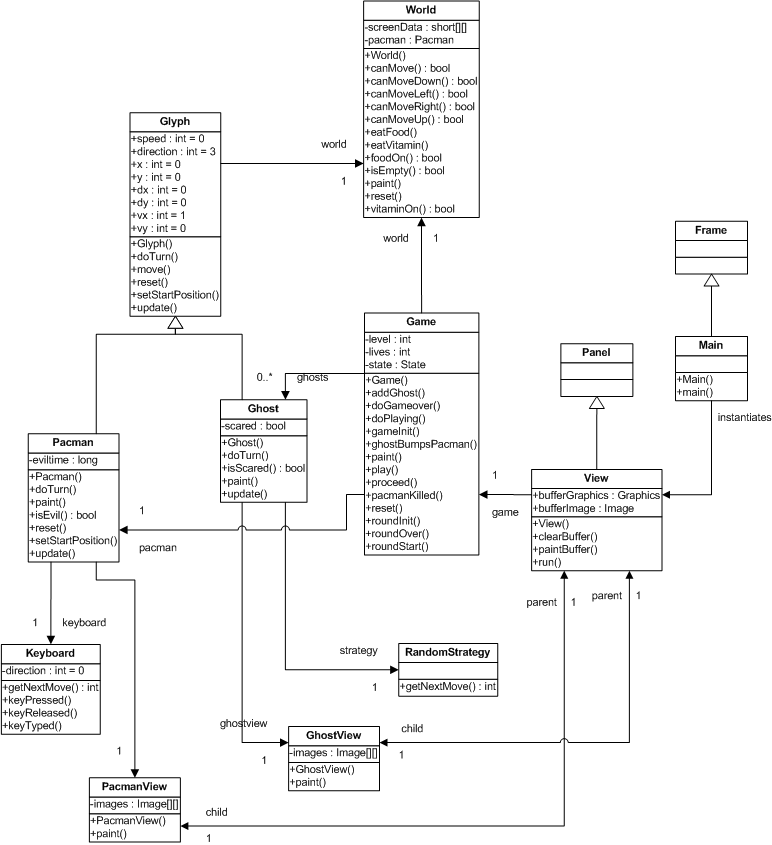
\includegraphics[style=page]{pacman_class_diagram}
  \caption{UML class diagram of the object-oriented Pacman game}
  \label{fig:pacman_class_diagram}
\end{figure}

\nomenclature{UML}{Unified Modeling Language}%
\autoref{fig:pacman_class_diagram} shows an initial object-oriented design for the Pacman game.
Note that this UML class diagram does not show the trivial accessors.
The classes in this diagram are:

%\begin{description}[noitemsep,style=sameline,leftmargin=38mm]
\begin{description}[noitemsep,style=nextline]
  \item [Game] This class encapsulates the control flow and controls the state of a game;
  \item [Ghost] This class is a representation of a ghost chasing pacman.
    Its main attribute is a property that indicates whether it is scared or not (depending on the evil state of pacman);
  \item [GhostView] This class is responsible for painting ghosts;
  \item [Glyph] This is the superclass of all mobile objects (pacman and ghosts).
    It contains common information like direction and speed;
  \item [Keyboard] This class accepts all keyboard input and makes it available to pacman;
  \item [Main] This is the entry point of a game;
  \item [Pacman] This is a representation of the user controlled element in the game.
    Its main attribute is a property that indicates whether pacman is evil or not;
  \item [PacmanView] This class is responsible for painting pacman;
  \item [RandomStrategy] By using this strategy, ghosts move in random directions;
  \item [View] This class is responsible for painting a maze;
  \item [World] This class has all the information about a maze.
    It knows where the vitamins, mega vitamins and most importantly the walls are.
    Every class derived from class \lstinline|Glyph| checks whether movement in the desired direction is possible.
\end{description}

\subsection{Completing the Pacman Example}
The initial object-oriented design, described in the previous section, does not implement all the stated system requirements.
The missing requirements are:

\begin{itemize}[noitemsep]
  \samepage
  \item The application does not maintain a score for the user;
  \item Ghosts move in random directions instead of chasing or fleeing from pacman.
\end{itemize}

In the next sections, we describe why and how to implement these requirements in the \Compose* language.

\subsubsection{Implementation of Scoring}
The first system requirement that we need to add to the existing Pacman game is scoring.
This concern involves a number of events.
First, the score should be set to zero when a game starts.
Second, the score should be updated whenever pacman eats a vitamin, mega vitamin or ghost.
And finally, the score itself has to be painted on the maze canvas to relay it back to the user.
These events scatter over multiple classes: \lstinline|Game| (initializing score), \lstinline|World| (updating score), \lstinline|Main| (painting score).
Thus scoring is an example of a crosscutting concern. 

To implement scoring in the \Compose* language, we divide the implementation into two parts.
The first part is a \Compose* concern definition stating which filter modules to superimpose.
\autoref{lst:scoringconcern} shows an example \Compose* concern definition of scoring.

\begin{lstlisting}[style=floatlisting,escapeinside={&$}{$&},language=ComposeStar,caption={\expandafter{\lstinline[style=inline]|DynamicScoring|} concern in \Compose*{}},label=lst:scoringconcern]
concern DynamicScoring in pacman {&$\label{line:dynscore_concern}$&
  filtermodule dynamicscoring {&$\label{line:dynscore_fm_begin}$&
    externals
      score : pacman.Score = pacman.Score.instance();
    inputfilters 
      score_filter : Meta = {[*.eatFood] score.eatFood,&$\label{line:score_filter}$&
                             [*.eatGhost] score.eatGhost,
                             [*.eatVitamin] score.eatVitamin,
                             [*.gameInit] score.initScore,
                             [*.setForeground] score.setupLabel}
  }&$\label{line:dynscore_fm_end}$&
  superimposition {&$\label{line:dynscore_si_begin}$&
    selectors
      scoring = { C | isClassWithNameInList(C, ['pacman.World',
                                 'pacman.Game', 'pacman.Main']) };
    filtermodules
      scoring <- dynamicscoring;
  }&$\label{line:dynscore_si_end}$&
}
\end{lstlisting}

This concern definition is called \lstinline|DynamicScoring| (line~\ref{line:dynscore_concern}) and contains two parts.
The first part is the declaration of a filter module called \lstinline|dynamicscoring| (lines~\ref{line:dynscore_fm_begin}--\ref{line:dynscore_fm_end}).
This filter module contains one \emph{meta filter} called \lstinline|score_filter| (line~\ref{line:score_filter}).
This filter intercepts five relevant calls and sends the message in a reified form to an instance of class \lstinline|Score|.
The final part of the concern definition is the superimposition part (lines~\ref{line:dynscore_si_begin}--\ref{line:dynscore_si_end}).
This part defines that the filter module \lstinline|dynamicscoring| is to be superimposed on the classes \lstinline|World|, \lstinline|Game| and \lstinline|Main|.

The final part of the scoring concern is the so-called \emph{implementation part}.
This part is defined by a class \lstinline|Score|.
\autoref{lst:scoreimpl} shows an example implementation of class \lstinline|Score|.
Instances of this class receive the messages sent by \lstinline|score_filter| and subsequently perform the events related to the scoring concern.
In this way, all scoring events are encapsulated in one class and one \Compose* concern definition. 

\begin{lstlisting}[style=floatlisting,language=Java,caption={Implementation of class \expandafter{\lstinline[style=inline]|Score|}},label=lst:scoreimpl]
import Composestar.Runtime.FLIRT.message.*;
import java.awt.*;

public class Score 
{
  private int score = -100;
  private static Score theScore = null;
  private Label label = new java.awt.Label("Score: 0");

  private Score() {}

  public static Score instance() {
    if(theScore == null) {
      theScore = new Score();
    }
    return theScore;
  }

  public void initScore(ReifiedMessage rm) {
    this.score = 0;
    label.setText("Score: "+score);
  }

  public void eatGhost(ReifiedMessage rm) {
    score += 25;
    label.setText("Score: "+score);
  }

  public void eatVitamin(ReifiedMessage rm) {
    score += 15;
    label.setText("Score: "+score);
  }

  public void eatFood(ReifiedMessage rm) {
    score += 5;
    label.setText("Score: "+score);
  }

  public void setupLabel(ReifiedMessage rm) {
    rm.proceed();
    label = new Label("Score: 0");
    label.setSize(15*View.BLOCKSIZE+20,15*View.BLOCKSIZE);
    Main main = (Main)Composestar.Runtime.FLIRT.message.MessageInfo
                                 .getMessageInfo().getTarget();
    main.add(label,BorderLayout.SOUTH);
  }
}
\end{lstlisting}

\subsubsection{Implementation of Dynamic Strategy}
The last system requirement that we need to implement is the dynamic strategy of ghosts.
This means that a ghost should, depending on the state of pacman, hunt or flee from pacman.
We can implement this concern by using the strategy design pattern.
However, in this way, we need to modify the existing code.
This is not the case when we use \Compose*{} \emph{dispatch filters}.
\autoref{lst:dynamicstrategyconcern} demonstrates this. 

\begin{lstlisting}[style=floatlisting,escapeinside={&$}{$&},language=Composestar,caption={\expandafter{\lstinline[style=inline]|DynamicStrategy|} concern in \Compose*{}},label=lst:dynamicstrategyconcern]
concern DynamicStrategy in pacman {
  filtermodule dynamicstrategy {
    internals
      stalk_strategy : pacman.Strategies.StalkerStrategy;
      flee_strategy : pacman.Strategies.FleeStrategy;   
    conditions
      pacmanIsEvil : pacman.Pacman.isEvil();
    inputfilters
      stalker_filter : Dispatch = {!pacmanIsEvil =>&$\label{line:stalker_filter}$&
                        [*.getNextMove] stalk_strategy.getNextMove};
      flee_filter : Dispatch = {&$\label{line:flee_filter}$&
                        [*.getNextMove] flee_strategy.getNextMove}
  }
  superimposition {
    selectors
      random = { C | isClassWithName(C,
                        'pacman.Strategies.RandomStrategy') };
    filtermodules
      random <- dynamicstrategy;
  }
}
\end{lstlisting}

This concern uses \emph{dispatch} filters to intercept calls to method \lstinline|RandomStrategy.getNextMove| and redirect them to either \lstinline|StalkerStrategy.getNextMove| or \lstinline|FleeStrategy.getNextMove|.
If pacman is not evil, the intercepted call matches the first filter, which dispatches the intercepted call to method \lstinline|StalkerStrategy.getNextMove| (line~\ref{line:stalker_filter}).
Otherwise, the intercepted call matches the second filter, which dispatches the intercepted call to method \lstinline|FleeStrategy.getNextMove| (line~\ref{line:flee_filter}).

